\chapter{Simulaci\'on de ebullici\'on en FC-72}

En los primeros cap\'itulos de esta tesis se introdujo, analiz\'o y valid\'o un modelo que permite reproducir adecuadamente una ecuaci\'on de energ\'ia para flujo multif\'asico, tomando como base una nueva \lbe{} con operador de colisi\'on MRT que debe ser resuelta en forma simult\'anea con otra \lbe{} hidrodin\'amica de la familia \pp{}. El desarrollo de este nuevo modelo no qued\'o restringido \'unicamente a la nueva ecuaci\'on y su justificaci\'on formal, sino que forma parte de una m\'etodolog\'ia de an\'alisis destinada a realizar simulaciones consistentes de transferencia de calor en flujo multif\'asico.

El nuevo modelo, en sus versiones D2Q9 y D3Q15, fue validado mediante la resoluci\'on de problemas en los que es posible obtener una soluci\'on anal\'itica. En estos \red{problemas}, en su mayor\'ia unidimensionales, fue posible discriminar diferentes aspectos de las ecuaciones macrosc\'opicas recuperadas, permitiendo desarrollar un an\'alisis de las \lbe{} desde un punto de vista global, que abarca aspectos fundamentales de las t\'ecnicas num\'ericas cl\'asicas como precisi\'on y consistencia. 

Esta metodolog\'ia de verificaci\'on consiste en un primer paso obligatorio en el proceso de validaci\'on de cualquier t\'ecnica num\'erica o modelo novedoso. Sin embargo, siempre que sea posible, este proceso debe completarse con la evaluaci\'on de situaciones m\'as complejas y que involucren una fenomenolog\'ia similar a la que se pretende resolver con la nueva t\'ecnica, tomando mediciones o resultados de simulaciones que puedan usarse para construir una base de comparaci\'on s\'olida.

En este aspecto, la representaci\'on de experimentos o simulaciones de ebullici\'on como parte de la validaci\'on resulta una tarea sumamente compleja. El modelo de lattice Boltzmann propuesto constituye un mecanismo alternativo para obtener la soluci\'on de ecuaciones diferenciales de conservaci\'on de masa, impulso y energ\'ia en flujo multif\'asico, y no involucra el modelado de caracter\'isticas microsc\'opicas del fen\'omeno de ebullici\'on que surgen de aquellos enfoques basados en las mayores escalas espaciales. Como de destaca en la extensa revisi\'on de Liang y Mudawar \cite{liang_review_2019}, la din\'amica de estos procesos no depende simplemente de las propiedades del fluido, sino que se encuentra fuertemente influenciada por las caracter\'isticas microsc\'opicas de la superficie calefactora. De esta manera, los aspectos macrosc\'opicos m\'as representativos, como temperatura o flujo de calor en la superficie, o tama\~no de las burbujas, presentan una fuerte dependencia con la cantidad y forma de los sitios de nucleaci\'on, porosidad y permeabilidad de la superficie, tensi\'on superficial y \'angulo de contacto. Por lo tanto, esta fuerte dependencia dificulta la selecci\'on de experimentos que puedan ser usados como casos de validaci\'on, ya que en muchas ocaciones no es posible determinar a priori estas propiedades que deben ser reproducidas num\'ericamente.

A pesar de estas restricciones inherentes al fen\'omeno, en los \'ultimos a\~nos se produjo un avance significativo en el desarrollo de microdispositivos para levar a cabo experimentos de ebullici\'on, permitiendo un notable control sobre los sitios de nucleaci\'on \cite{gregorcic_scalable_2018, liu_experimental_2019}. De esta manera, la incorporaci\'on de sensores exclusivamente en la zona de generaci\'on de las burbujas y el uso de c\'amaras de alta velocidad y resoluci\'on, permitieron lograr una reconstrucci\'on detallada de procesos elusivos, como la formaci\'on, crecimiento y desprendimiento de burbujas individuales. En este l\'inea, Hutter y colaboradores \cite{hutter_experimental_2009,hutter_experimental_2010} lograron medir experimentalmente di\'ametro de burbujas en funci\'on del tiempo, frecuencia, di\'ametro de partida y tiempo de espera, en la ebullici\'on de FC72 sobre obleas de silicio con un n\'umero reducido de cavidades microfabricadas. 

Las caracter\'isticas de estas mediciones, en las que se reducen las incertezas asociadas a la descripci\'on de la superficie y se logra determinar con precisi\'on aquellas caracter\'isticas del flujo reproducibles con lattice Boltzmann, las convierten en un caso de validaci\'on ideal para el modelo propuesto en esta tesis. Por lo tanto, el presente cap\'itulo estar\'a dedicado a la reproducci\'on del experimento de ebullici\'on de Hutter mediante la aplicaci\'on del modelo y de la metodolog\'ia de an\'alisis desarrollada en los cap\'itulos anteriores.

\red{Decir en alg\'un punto que se trata de ebullici\'on nucleada}




\section{Descripci\'on del experimento}

El cuerpo principal del dispositivo experimental de Hutter \cite{hutter_experimental_2010} est\'a compuesto por una c\'amara de ebullici\'on de acero inoxidable, con cuatro ventanas de vidrio \red{borosilicato}, que permiten el acceso \'optico al substrato de ebullici\'on. Esta c\'amara se encuentra recubierta con calefactores aislados con silicona que permiten reducir la p\'erdida de calor hacia el ambiente, y contiene cuatro cartuchos calafactores utilizados para la desgasificaci\'on del \red{boiling l\'iquid} y para calefaccionarlo hasta alcanzar la temperatura de saturaci\'on. La c\'amara se encuentra conectada a un condensador externo, el cual es responsable de regular la presi\'on del sistema mientras que permite la recuperaci\'on del l\'iquido evaporado y su posterior regreso a la c\'amara principal.

El componente responsable de la ebullici\'on consiste en un chip de silicio, construido sobre una oblea de 3 pulgadas de di\'ametro y 380 $\mu m$ de espesor. En la \fig{fig:chip} se esquematiza el proceso de construcci\'on del chip: en uno de sus caras se produce una capa de di\'oxido de silicio que contiene en su interior a los sensores de temperatura y el circuito calefactor de Al, mientras que en la superficie restante se generan las microcavidades que actuar\'an como sitios de nucleaci\'on.

\begin{figure}[ht]
	\centering
	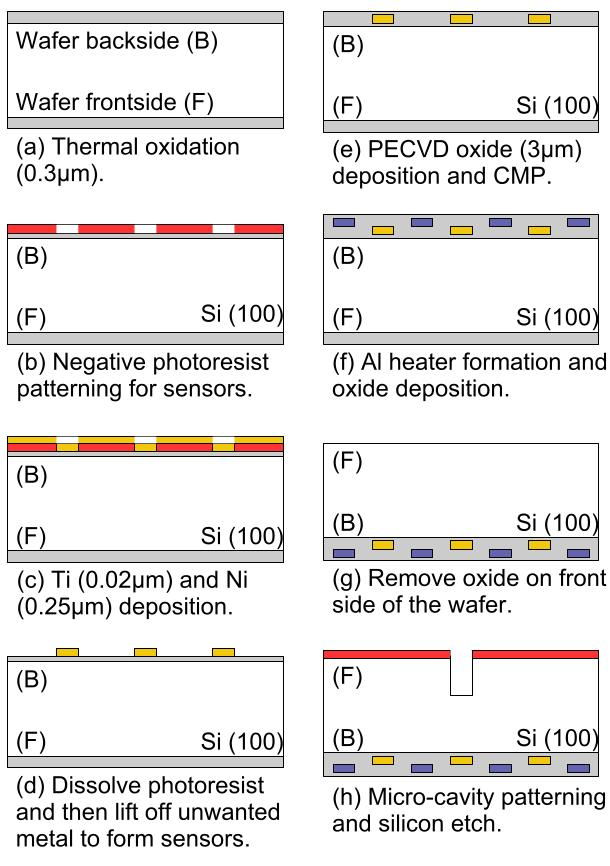
\includegraphics[width=0.5\textwidth]{FC72/Substrate}
	\caption{Secuencia de fabricaci\'on del chip de ebullici\'on, que contiene las microcavidades, los sensores de temperatura integrados (amarillo), y la resistencia calefactora integrada (azul). Reimpreso de \cite{hutter_experimental_2010}.}
	\label{fig:chip}
\end{figure}

Las cavidades artificiales fueron generadas sobre la placa de silicio mediante un proceso de grabado profundo con iones activos (\emph{deep reactive ion etching}), y corresponden a peque\~nos orificios de 40 $\mu m$ de profundidad y 10 $\mu m$ de di\'ametro. Como se muestra en la \fig{fig:cavidad}, esta t\'ecnica permite generar cavidades con formas precisas, claramente distinguibles de la rugosidad superficial del chip.

\begin{figure}[ht]
	\centering
	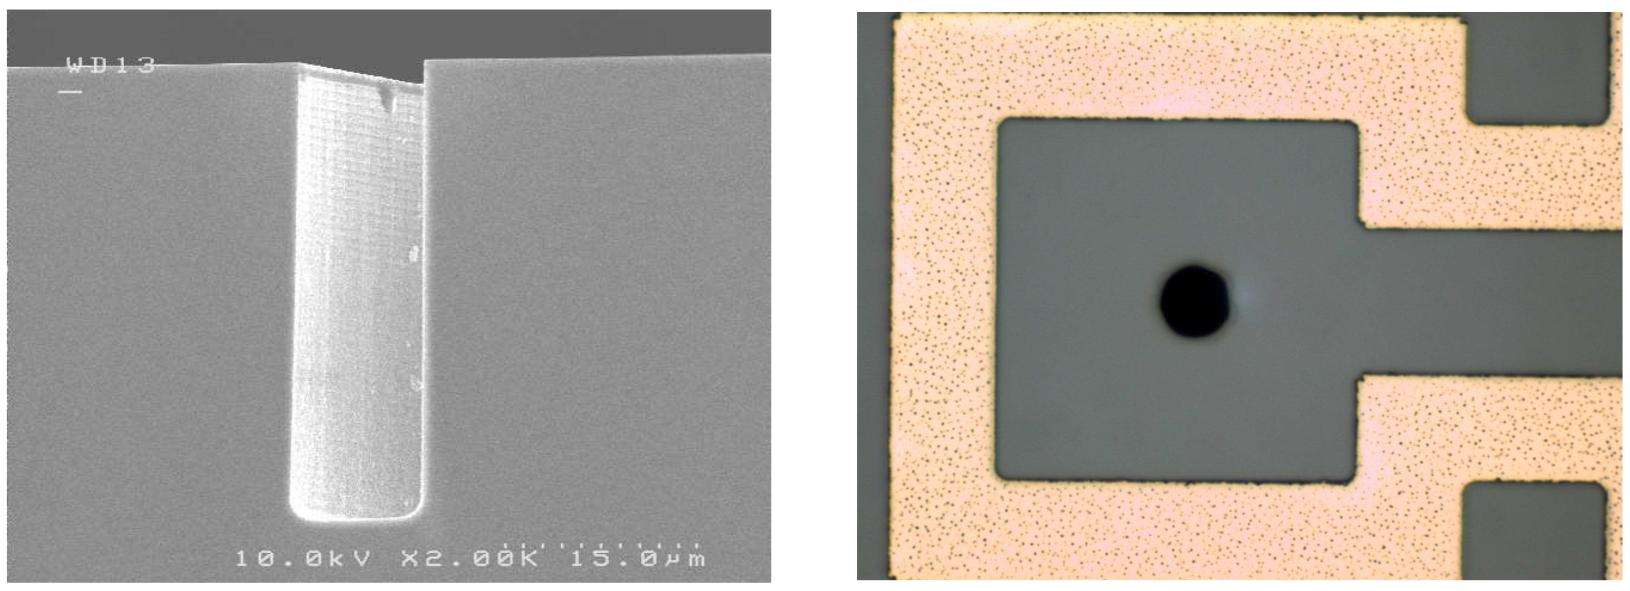
\includegraphics[width=0.75\textwidth]{FC72/Cavity}
	\caption{Izquierda: imagen SEM de una secci\'on a trav\'es de una cavidad elongada. Derecha: imagen de la apertura de la cavidad.}
	\label{fig:cavidad}
\end{figure}


\subsubsection{\red{Boiling liquid}}

El fluido de trabajo utilizado fue perfluorohexano C$_6$F$_14$, conocido comercialmente como Fluorinert FC-72. Es un l\'iquido claro, incoloro, t\'ermica y qu\'imicamente estable, compatible con materiales sensibles, inflamable, poco t\'oxico y ampliamente utilizado en experimentos de ebullici\'on. Su baja temperatura de ebullici\'on ($T_{sat}=57.15$ \textordmasculine C a 1 atm de presi\'on) y sus propiedades diel\'ectricas permiten sumergir completamente las conexiones el\'ectricas de la c\'amara y el chip calefactor.  \red{Algo m\'as}


El di\'ametro de las burbujas pudo ser medido a partir de im\'agenes capturadas por una c\'amara de alta velocidad, y corresponde al m\'aximo di\'ametro aparente o ecuador de las mismas. En la \fig{fig:sequence} se muestra una secuencia de im\'agenes con una resoluci\'on temporal de 6 ms para el crecimiento de una burbuja en una cavidad de 80 $\mu$m de profundidad y 10 $\mu$m de di\'ametro, con un exceso de temperatura de 1.1 K en la superfcie calefactora (respecto a la temperatura de saturaci\'on) y 1.25 atm de presi\'on.

\begin{figure}[ht]
	\centering
	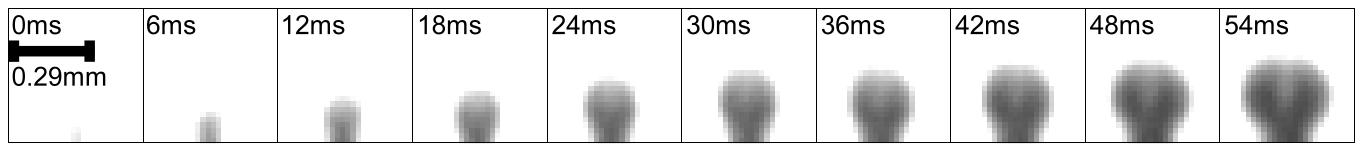
\includegraphics[width=0.9\textwidth]{FC72/sequence}
	\caption{Im\'agenes de alta velocidad de la secuencia de crecimiento de una burbuja en una cavidad aislada.}
	\label{fig:sequence}
\end{figure}





\section{Modelo num\'erico}

\subsection{Selecci\'on de los par\'ametros de simulaci\'on}

Las mediciones realizadas por Hutter permitieron cuantificar la evoluci\'on del di\'ametro de burbuja aparente, desde la formaci\'on hasta el desprendimiento de cada burbuja individual, bajo condiciones de ebullici\'on saturada de FC-72 a diferentes presiones. Sin embargo, como se detalla en el \chap{chap:modelo2D}, la naturaleza adimensional del formalismo utilizado no permite realizar una construcci\'on directa del dominio computacional para este problema, sino que es necesario impulsar la elecci\'on de modelos computacionales que simulen los mismos n\'umeros adimensionales representativos del experimento. Por otro lado, adem\'as de las ventajas provenientes de la adimensionalizaci\'on, es necesario tener en cuenta la consistencia observada en las soluciones num\'ericas si se expresa en unidades adimensionales, ya que las interfases recuperadas tienen un espesor que depende de las constantes de estado, y que es fijo en unidades de grilla.

De acuerdo a las ecuaciones recuperadas por las \lbe{}, estos par\'ametros adimensionales corresponden a:
\begin{equation}
	Re = \dfrac{\rho_l g^{1/2} D^{3/2}}{\mu_l}, \qquad
	Bo = \dfrac{\rho_l g D^2}{\kappa}, \qquad
	Pr = \dfrac{\nu}{\alpha}, \qquad
	Ja = \dfrac{c_v}{h_{fg}}(T_w-T_s),
	\label{eq:num_adim_hetb_3D}
\end{equation}
donde $Re$, $Bo$, $Ja$ y $Pr$ son los n\'umeros de Reynolds, Bond, Jacob y Prandtl respectivamente. En la \eq{eq:num_adim_hetb_3D} $D$ corresponde a una dimension caracter\'istica, $\mu_l$ a la viscosidad din\'amica de la fase l\'iquida, $\kappa$ a la tensi\'on superficial, y $T_w$ y $T_s$ corresponden a la temperatura sobre la pared y en el seno del fluido, respectivamente. Como en el modelo propuesto en el \chap{chap:modelo3D} no es posible fijar el calor latente y tensi\'on superficial, sino que corresponden a propiedades recuperadas dependientes de las dem\'as constantes de simulaci\'on, puede usarse la \eq{eq:num_adim_hetb_3D} para fijar los par\'ametros restantes:
\begin{equation}
	g = \dfrac{Bo \kappa}{\rho_l D^2}, \qquad
	\nu_l = \dfrac{g^{1/2}D^{3/2}}{Re} = \sqrt{ \dfrac{Bo \kappa D}{\rho_l Re^2} }, \qquad
	\alpha = \dfrac{\nu}{Pr}, \qquad
	c_v = \dfrac{Ja h_{fg}}{(T_w - T_s)}.
	\label{eq:param_adim_3D}
\end{equation}


Estas condiciones, sumadas a la experiencia adquirida durante el desarrollo del modelo y las etapas previas de validaci\'on, llevan a proponer la realizaci\'on de un conjunto de pasos previos a la simulaci\'on del experimento, con el objetivo de determinar las constantes de simulaci\'on decuadas. De esta manera, la evaluaci\'on preliminar para la simulaci\'on con modelos \pp{} debe seguir el siguiente camino:
\begin{enumerate}
	\item C\'alculo de los n\'umeros adimensionales del experimento.
	\item Selecci\'on de la ecuaci\'on de estado.
	\item Determinaci\'on de constantes de estado adecuadas. \label{it:eos_const}
	\item C\'alculo de tensi\'on superficial recuperada.
	\item C\'alculo de calor latente recuperado.
	\item C\'alculo de factores de relajaci\'on y dem\'as constantes de la simulaci\'on.
	\item Revisi\'on desde el paso \ref{it:eos_const} hasta encontrar una combinaci\'on de factores satisfactoria.
\end{enumerate}


\subsubsection{N\'umeros adimensionales del experimento}

La determinaci\'on de los n\'umeros adimensionales no es \'unica, ya que depende, entre otros factores, de la elecci\'on de una longitud caracer\'istica $D$. En este caso se desea reproducir la generaci\'on de burbujas en un \'unico sitio de nucleaci\'on, empleando un dominio computacional prism\'atico con el mayor tama\~no posible, con el objetivo de reducir los efectos de la frontera sobre la din\'amica de las burbujas. Por lo tanto, resulta natural tomar como $D$ a alguna de las dimensiones principales de la microcavidad, como di\'ametro o profundidad. Sin embargo, una estimaci\'on preliminar de la cantidad necesaria de unidades de grilla para lograr una adecuada descripci\'on de cada burbuja, muestra que con la capacidad de c\'alculo disponible para el desarrollo de esta tesis, no es posible discretizar adecuadamente la totalidad de la cavidad. Por lo tanto, se decide representar a $D$ como el di\'ametro aparente de las burbujas, teniendo en cuenta que, para las simulaciones, este par\'ametro es un resultado del c\'alculo y no un valor preestablecido.

Las mediciones de Hutter que ser\'an empleadas en esta comparaci\'on muestran que el di\'ametro de partida observado es $D_p=0.33$ mm, con lo que se obtienen los n\'umeros adimensionales detallados en la \tb{tab:exp_adim}
\begin{table}[ht]
	\centering
    \begin{tabular}{c c}
	    \toprule
		Re & $66.998$  \\
		Bo & $0.20927$ \\
		Pr & $9.5497$ \\
		Ja & $0.016892$ \\
        \bottomrule
	\end{tabular}
	\caption{N\'umeros adimensionales del experimento de ebullici\'on de Hutter.}
	\label{tab:exp_adim}
\end{table} 


\subsubsection{Selecci\'on de la ecuaci\'on de estado}

Para esta etapa es necesario encontrar una ecuaci\'on de estado de reproduzca adecuadamente la curva de coexistencia ($T_r - \rho_r$) del FC-72. A diferencia de lo que ocurre con otros refrigerantes, las propiedades del FC-72 no se encuentran incluidas en bases de datos abiertas, por lo que se han extra\'ido de la tesis de Geisler \cite{larson_geisler_buoyancy-driven_2007} y del trabajo de Cao \cite{cao_experimental_2019}. En la \tb{tab:fc72_prop} se resumen las caracter\'isticas necesarias para la simulaci\'on, calculadas a temperatura de saturaci\'on ($329.75$ K) y presi\'on atmosf\'erica.

\begin{table}[ht]
	\centering
    \begin{tabular}{c c c c}
	    \toprule
        \bf Propiedad & \bf Notaci\'on & \bf Valor (SI)\\
        \midrule
		Temperatura de saturaci\'on & $T_s$ & $329.75$ K \\
		Temperatura de saturaci\'on reducida & $T_{s_r}$ & $0.73474$ \\
		Densidad de l\'iquida & $\rho_l$ & $1620$ kg/m\sps{3} \\
		Densidad de vapor & $\rho_g$ & $13.4$ kg/m\sps{3} \\		
		Viscosidad de l\'iquido & $\nu_l$ & $2.8025 \, \cdot\,10^{-7}$ kg/(m s) \\		
		Viscosidad de vapor & $\nu_g$ & $8.9552 \, \cdot\,10^{-7}$ kg/(m s) \\
		Tensi\'on superficial & $\sigma_s$ & $0.00827$ N/m \\
		Cond. t\'ermica l\'iquido & $\lambda_l$ & $0.0522$ W/(m K) \\
		Cond. t\'ermica vapor & $\lambda_l$ & $0.0129$ W/(m K) \\
		Calor espec\'ifico l\'iquido & $c_{v_l}$ & $1098$ J/(kg K) \\
		Calor espec\'ifico vapor & $c_{v_g}$ & $894$ J/(kg K) \\
		Calor latente & $h_{fg}$ & $84500$ \red{J/(kg K)} \\
        \bottomrule
	\end{tabular}
	\caption{Propiedades principales de FC-72 a $p=1$ atm y $T=329.75$ K.}
	\label{tab:mx3D_prop}
\end{table} 
\FloatBarrier

Los experimentos analizados fueron realizados principalmente a presi\'on atmosf\'erica, de modo que el objetivo de esta etapa se reduce a identificar la ecuaci\'on de estado que mejor reproduce la relaci\'on de densidades a la temperatura reducida correspondiente a esta condici\'on de saturaci\'on. En la \fig{fig:eos_fc72} se muestran las curvas de coexistencia correspondientes a las ecuaciones de estado de van der Waals, Carnahan-Starling (\eq{eq:CS_eos}) y Peng-Robinson (\eq{eq:PR_eos}), junto con las densidades de coexistencia de FC-72 a presi\'on atmosf\'erica. En este caso, puede  verse que la \'unica ecuaci\'on capaz de producir satisfactoriamente las densidades de coexistencia a la temperatura deseada es la de Peng-Robinson, con un factor de excentricidad $\omega=0.5$.

\begin{figure}[ht]
	\centering
	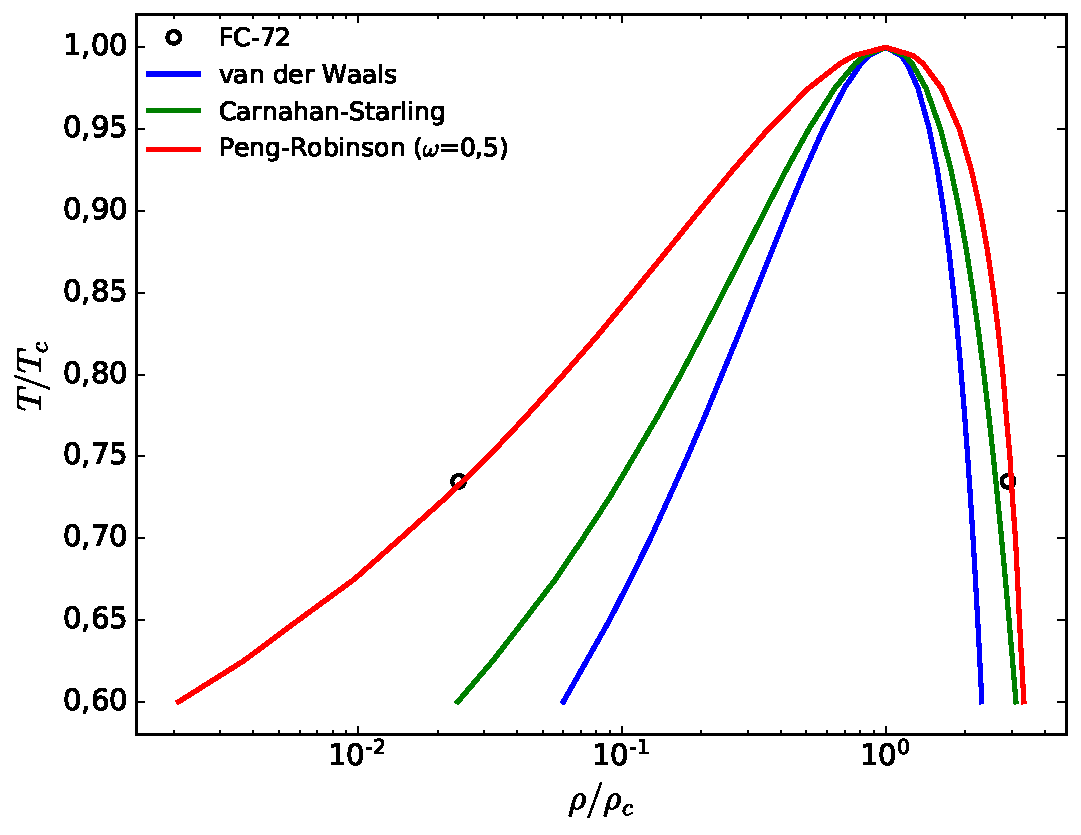
\includegraphics[width=0.75\textwidth]{FC72/EOS/EOS_FC72}
	\caption{Ecuaciones de estado y densidades de coexistencia para FC72.}
	\label{fig:eos_fc72}
\end{figure}


\subsubsection{Determinaci\'on de las constantes de estado}

En la \fig{fig:eos_fc72} se observa que la ecuaci\'on de estado de Peng-Robinson con $\omega=0.5$ es capaz de reproducir la relaci\'on de densidades requerida ($\rho_l/\rho_g = 120.9$) a una temperatura reducida cercana a la del experimento ($T_{s_r}=0.73474$). Espec\'ificamente, mediante un proceso de minimizaci\'on puede verse que esta ecuaci\'on de estado alcanza la relaci\'on de densidades buscada para $T_r=0.73438$.

Por otro lado, las curvas de coexistencia de la \fig{fig:eos_fc72} est\'an expresadas en unidades reducidas, lo que implica que a\'un es necesario elegir un conjunto de constantes ($a$, $b$) admisibles, es decir, que conduzcan a simulaciones estables. Como se mostr\'o en las Secciones~\ref{sec:vdw_1d} y \ref{sec:vdWColumnHT}, las constantes de estado determinan los valores absolutos de densidades y temperatura reproducidas (no reducidas), as\'i como el espesor de la interfase en unidades de grilla. Por lo tanto, el criterio de selecci\'on para este problema consiste en elegir  un conjunto de constantes que, para $T_r=0.73438$, reproduzcan una interfase con 5-10 unidades de grilla.

La evaluaci\'on del perfil de densidad a trav\'es de la interfase se llev\'o a cabo en dominios similares a los usados para el c\'alculo de tensi\'on superficial, simulando la evoluci\'on de una burbuja estacionaria de 100 u.g de di\'ametro dentro de una cavidad c\'ubica y peri\'odica con $200 \times 200 \times 200$ u.g. Mediante este proceso se seleccionaron las constantes $a=1/50$ y $b=2/21$, las cuales repoducen una interfase de 9 u.g. con $\sigma=0.125$, como se muestra en la \fig{fig:rho_int_bubble}.
\begin{figure}[ht]
	\centering
	
\includegraphics[width=0.75\textwidth]{dummy}
	\caption{Perfil de densidad a trav\'es de la interfase de una burbuja estacionaria, calculada para $T_r=0.73438$ usando la ecuaci\'on de Peng-Robinson con $a=1/50$, $b=2/21$ y $\omega=0.5$.}
	\label{fig:rho_int_bubble}
\end{figure}



\subsubsection{C\'alculo de tensi\'on superficial}

Una vez definidas las constantes de la ecuaci\'on de estado, es posible determinar la tensi\'on superficial recuperada mediante esperimentos num\'ericos para evaluar la Ley de Laplace. Para ello, se simul\'o la evoluci\'on de burbujas estacionarias, ubicadas en el centro de una cavidad c\'ubica de $200 \times 200 \times 200$ u.g. con condiciones de contorno peri\'odicas en todas sus caras. Inicialmente, estas burbujas est\'an compuestas por un fluido de densidad $\rho_g$ dentro de una matriz de densidad $\rho_l$, donde $\rho_g$ y $\rho_l$ corresponden a las densidades de coexistencia de las fases de vapor y l\'iquido a $T_r$ respectivamente.

De acuerdo al modelo hidrodin\'amico de Xu la presi\'on en cada nodo puede calcularse mediante la \eq{eq:PTens_Xu}, de modo que si se simulan burbujas con diferente radio inicial, la tensi\'on superficial puede calcularse usando una regresi\'on lineal para la ecuaci\'on de Laplace:
\begin{equation}
	p_{in}-p_{out} = \dfrac{\sigma_s}{2 R},
\end{equation}
donde $p_{in}$ y $p_{out}$ corresponden al valor de presi\'on en el interior y exterior de la burbuja respectivamente, lejos de la interfase. A modo de ejemplo, en la \fig{fig:laplace_1_3D} se muestran los resultados de la evoluci\'on de la burbuja estacionaria, donde puede observarse la distribuci\'on final de densidad y magnitud de valocidad (en este caso son corrientes esp\'ureas), as\'i como el perfil de presi\'on a lo largo de la direcci\'on $x$, tomando como origen el centro de la burbuja.
\begin{figure}[htb]
    \centering
    \begin{subfigure}[t]{0.45\textwidth}
        \centering
        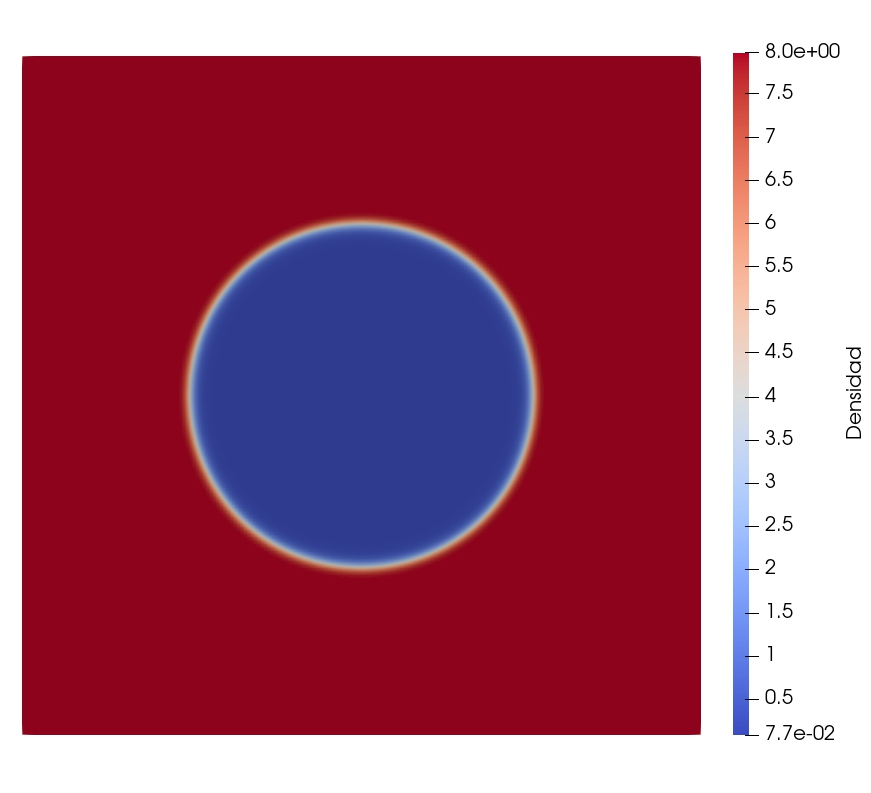
\includegraphics[width=0.95\textwidth]{FC72/LaplaceLaw/Densidad_PlanoZ}
        \caption{Densidad sobre un plano con origen en el centro de la burbuja.}
    \end{subfigure}
    \begin{subfigure}[t]{0.45\textwidth}
        \centering
        \includegraphics[width=0.95\textwidth]{FC72/LaplaceLaw/Velocidad_PlanoZ}
        \caption{Magnitud de velocidad sobre un plano con origen en el centro de la burbuja.}
    \end{subfigure}
    \begin{subfigure}[t]{0.45\textwidth}
        \centering
        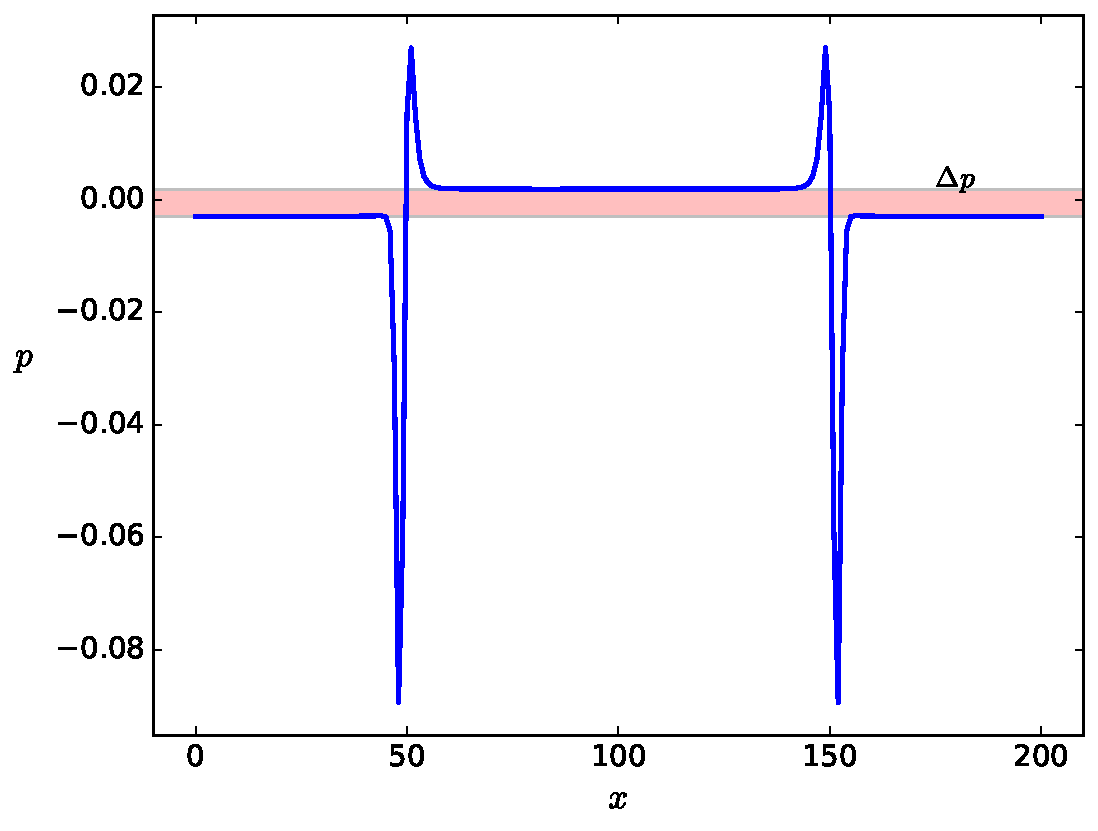
\includegraphics[width=0.95\textwidth]{FC72/LaplaceLaw/pressure_xaxis}
        \caption{Distribuci\'on de presi\'on  a trav\'es de una burbuja estacionaria.}
    \end{subfigure}    
    \caption{Ejemplo de burbuja estacionaria empleada en la simulaci\'on de la ley de Laplace.}
    \label{fig:laplace_1_3D}
\end{figure}

El esquema isot\'ermico de Xu incorpora un t\'ermino de fuente adicional que permite modificar la tensi\'on superficial recuperada mediante cambios en el par\'ametro libre $\kappa$. En la \fig{fig:delta_p_kappa} se muestran los resultados del experimento num\'erico de Ley de Laplace, donde se deja evolucionar un conjunto de burbujas de diferente radio inicial y se mide la presi\'on interna y externa despu\'es de alcanzado un estado estacionario. Como puede observarse, esta diferencia de presiones var\'ia linealmente con $1/R$, donde $R$ es el radio final medido para cada burbuja, y la pendiente de este ajuste ($\sigma_s$) depende del valor de $\kappa$ utilizado.

\begin{figure}[ht]
	\centering
	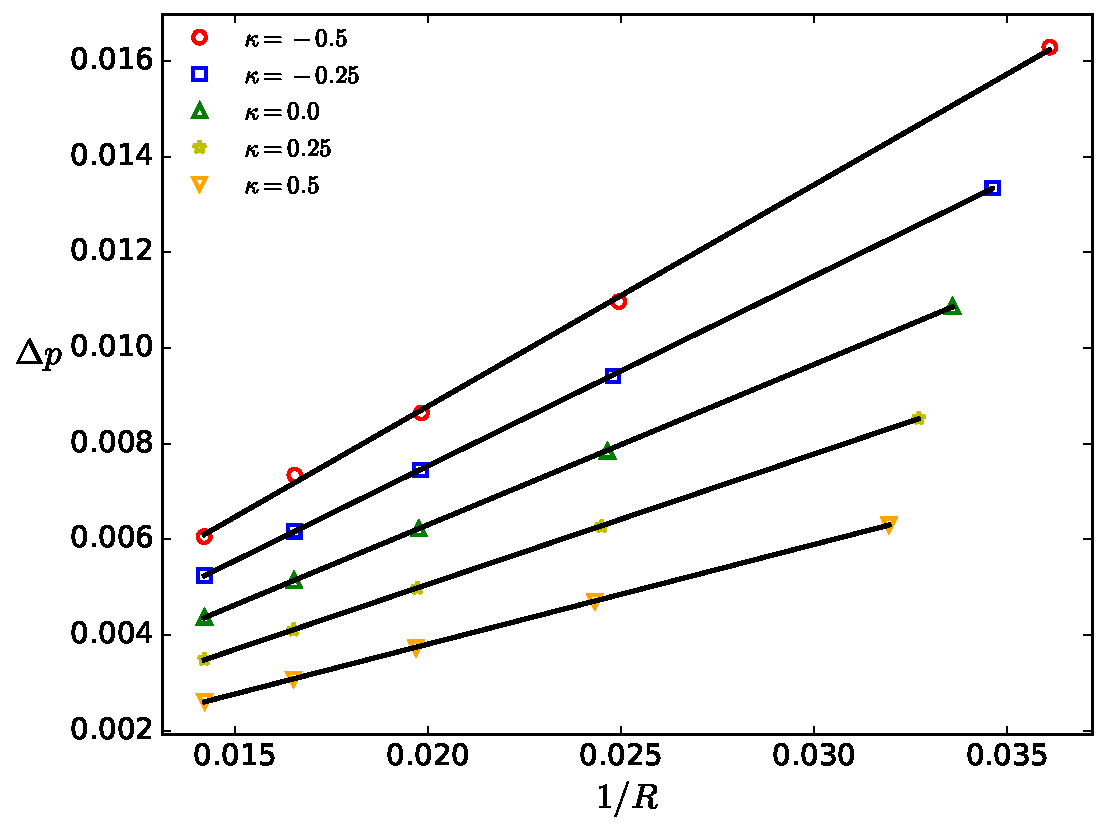
\includegraphics[width=0.75\textwidth]{FC72/LaplaceLaw/pressure_kappa}
	\caption{Experimento num\'erico de Ley de Laplace para diferentes valores de $\kappa$.}
	\label{fig:delta_p_kappa}
\end{figure}

El an\'alisis de los n\'umeros adimensionales de la \eq{eq:num_adim_hetb_3D} muestra que si se desea subir la viscosidad del fluido simulado para alejar a los factores de relajaci\'on de los l\'imites de estabilidad, entonces es necesario incrementar los valores de tensi\'on superficial recuperada. Por lo tanto, esto implica emplear un valor de $kappa$ negativo, con el mayor m\'odulo posible. En este caso, con las constantes de estados previamente elegidas se alcanzaron simulaciones estables con $\kappa=-0.5$.

Los resultados que se observan en la \fig{fig:delta_p_kappa} fueron obtenidos con los factores de relajaci\'on que se detallan en la \tb{tab:vdwColumn3D_prop}, con $\tau_{\nu}^{-1}=1.0$. Sin embargo, es necesario destacar que a pesar que el modelo de Xu no produce desviaciones significativas en las densidades de coexistencia para diferentes valores de $\tau_{\nu}$, s\'i se han observado cambios en la tensi\'on superficial recuperada. Por lo tanto, durante el proceso de selecci\'on de constantes de simulaci\'on adecuadas, debe repetirse este experimento si se modifican los factores de relajaci\'on.


\subsubsection{C\'alculo de calor latente recuperado}

En los Cap\'itulos~\ref{chap:modelo2D} y \ref{chap:modelo3D} se verific\'o, mediante la simulaci\'on del problema de Stefan unidimensional, que el calor latente recuperado queda determinado por la ecuaci\'on de estado utilizada. Sin embargo, pueden surgir discrepancias con la soluci\'on anal\'itica cuando se utilizan, por ejemplo, factores de relajaci\'on  diferentes en cada fase (para cualquiera de las \lbe{}). Por lo tanto, resulta conveniente medir el calor latente recuperado a trav\'es de un experimento num\'erico sencillo.

Tomando como base los trabajos de Fang \cite{fang_lattice_2017} y Zhang \cite{zhang_simulation_2015}, se eligi\'o la construcci\'on de un experimento num\'erico que consiste en un dominio de $L=150$ u.g. en la direcci\'on $x$ y s\'olo $H=3$ en las direcciones peri\'odicas $z$ e $y$, similar al empleado en la simulaci\'on del problema de Stefan. Sin embargo, a diferencia del frente de evaporaci\'on, el nuevo dominio contiene inicialmente un fluido en reposo a temperatura $T_{s_r}$, con $\rho_l$ para $x<0.5L$ y $\rho_l$ para $x>0.5L$. Si en este caso se impone un flujo de calor constante en el extremo cerrado de la cavidad ($x=0$), entonces es posible calcular el calor latente a partir de la medici\'on del cambio de masa:
\begin{equation}
	q = m'' h_{fg},
\end{equation}
donde $q$ es la potencia entregada durante un cierto tiempo de simulaci\'on y $m''$ la masa de l\'iquido evaporada durante ese per\'iodo. De esta manera, puede obtenerse una estimaci\'on de $h_{fg}$ mediante el ajuste lineal del cambio de masa obtenido para diferentes flujos de calor, como se ejemplifica en la \fig{fig:calor_latente_3D}. En este caso, el calor latente recuperado para $\tau_{\nu}^{-1}=1.0$, $a=1/50$ y $b=2/21$ corresponde $h_{fg}=0.26$, mientras que el anal\'itico para la ecuaci\'on de Peng-Robinson \cite{peng_new_1976} es de $h_{fg}=0.24$.

\begin{figure}[ht]
	\centering
	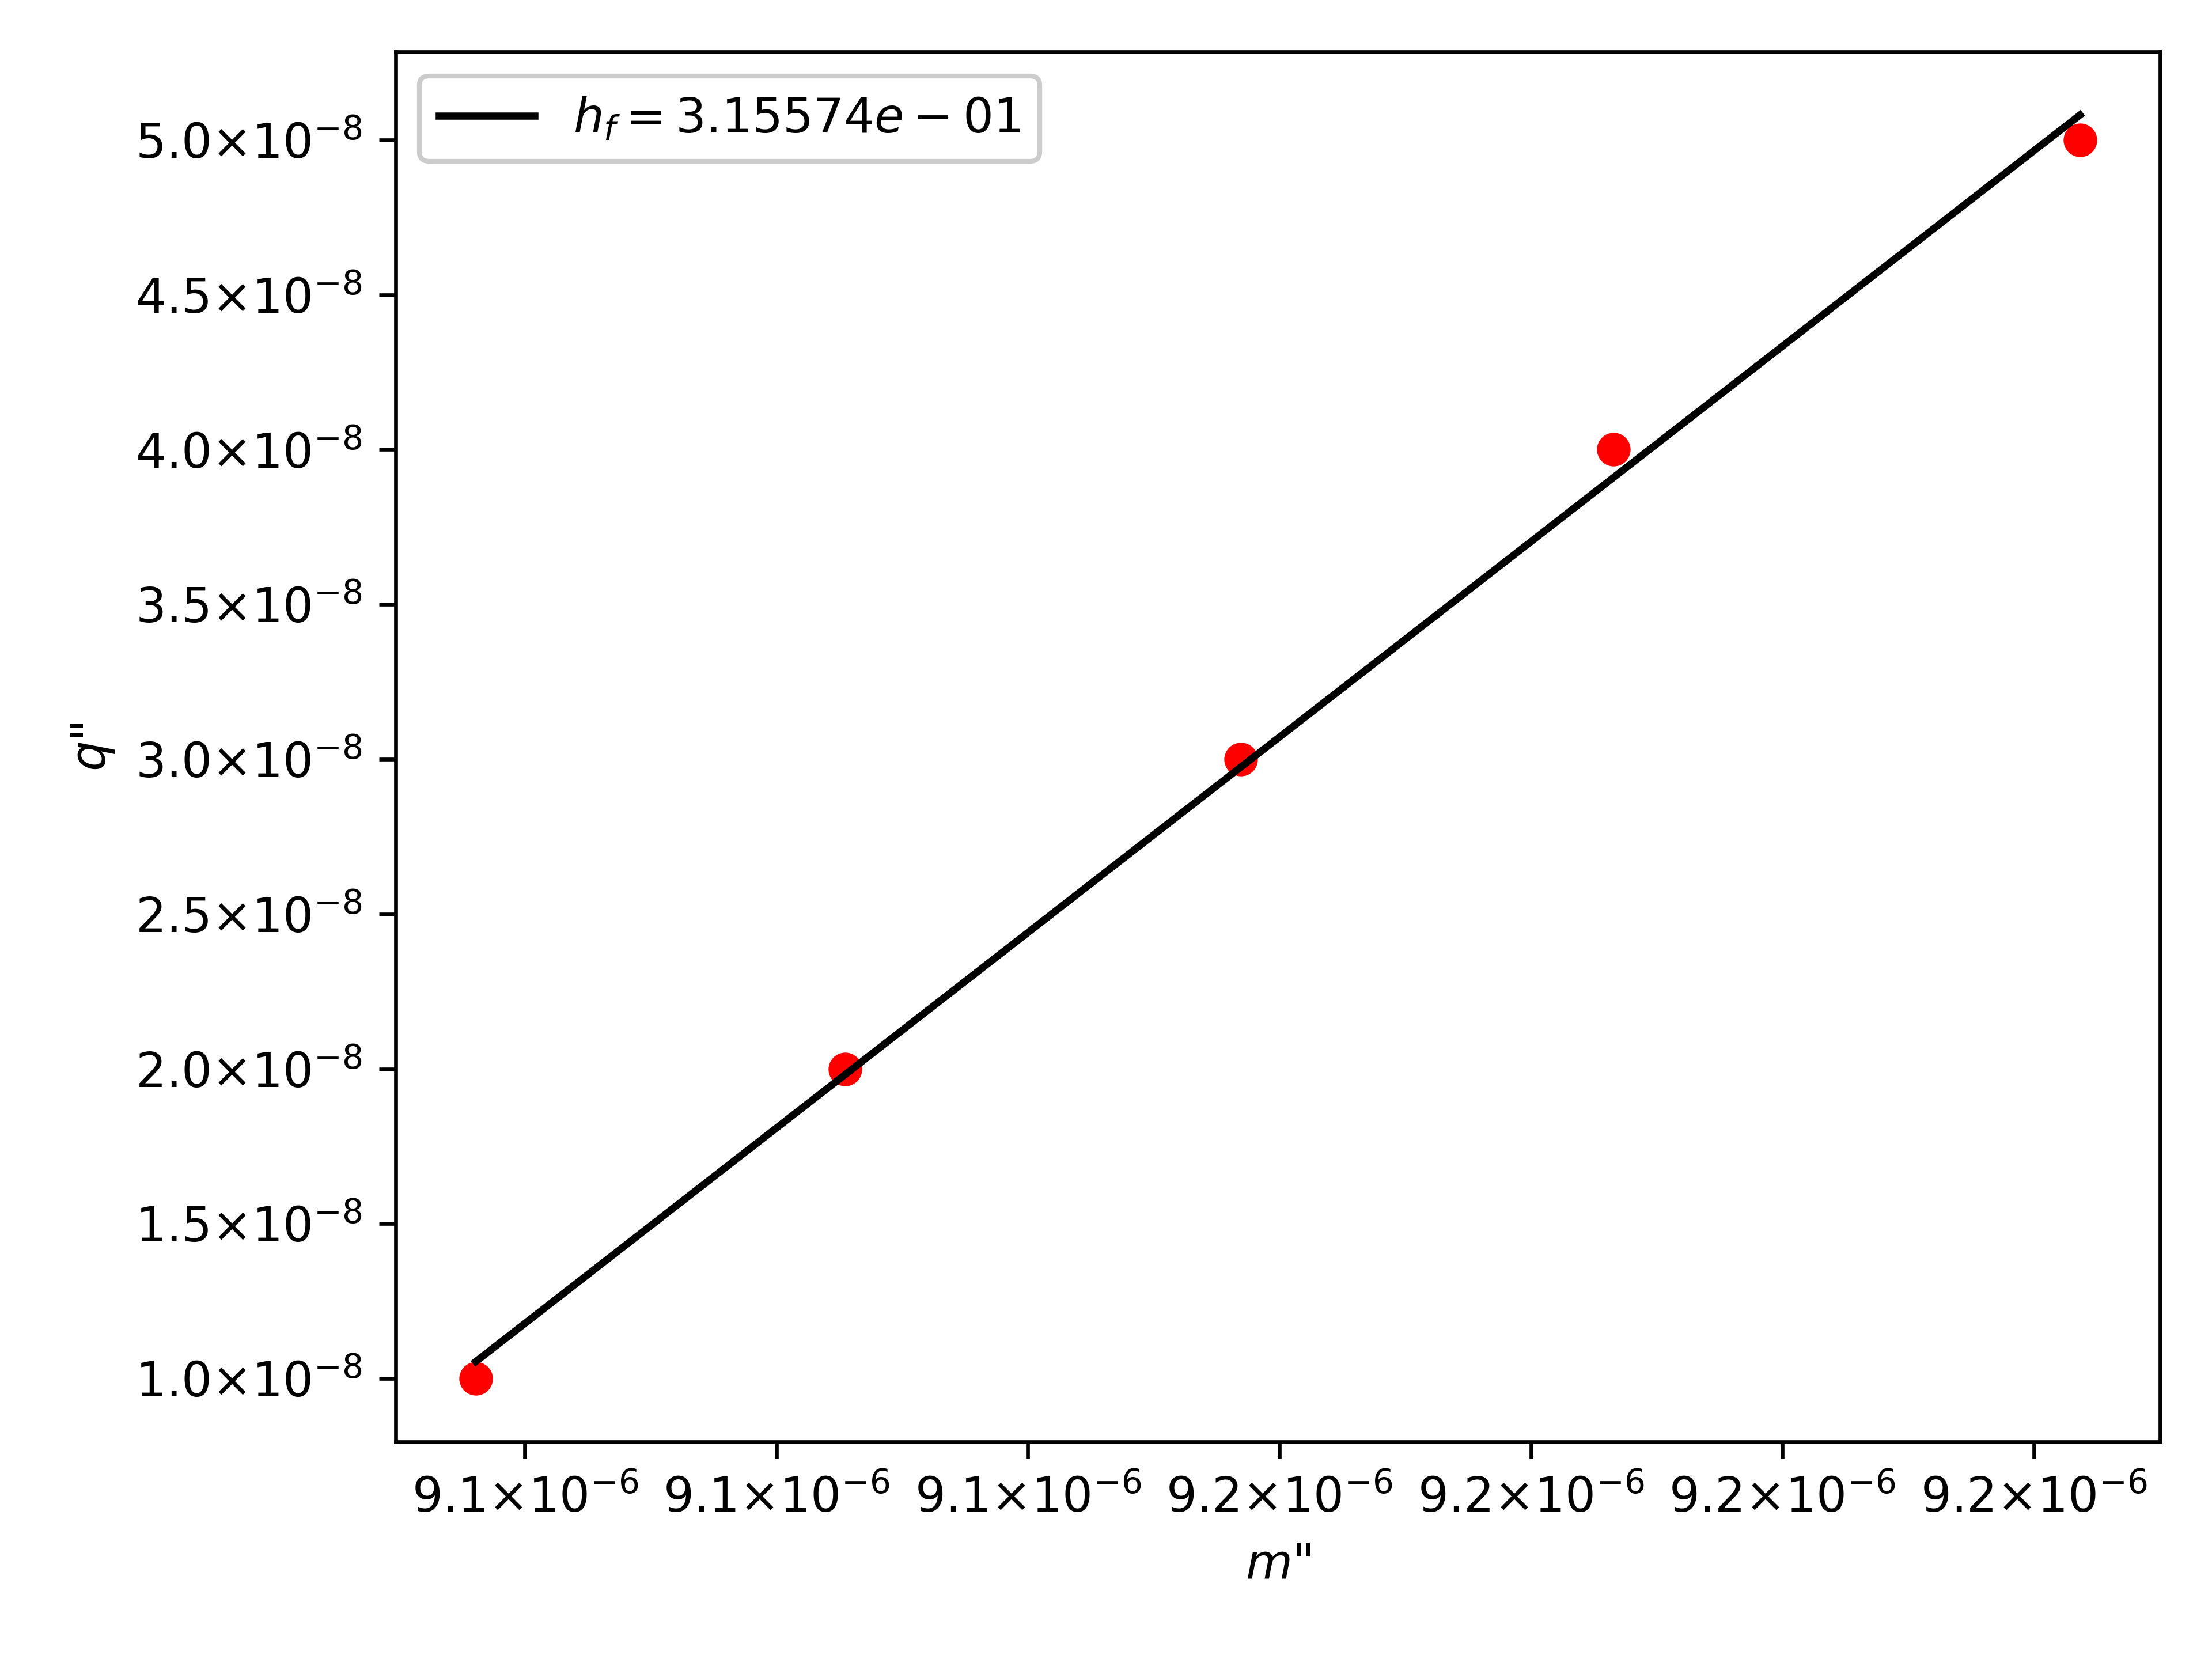
\includegraphics[width=0.75\textwidth]{FC72/latentHeat/latentHeat}
	\caption{Experimento num\'erico para la determinaci\'on del calor latente.}
	\label{fig:calor_latente_3D}
\end{figure}


\subsubsection{C\'alculo de factores de relajaci\'on y dem\'as constantes de la simulaci\'on}

Una vez determinadas aquellas propiedades macrosc\'opicas recuperadas, como tensi\'on superficial y calor latente, resta definir $\alpha_1$ y $\alpha_2$ para completar el c\'alculo de la difusividad t\'ermica, y por lo tanto de $q_{\chi}$ necesario. Para ello, es necesario encontrar un conjunto que permita reducir $q_{\chi}$ todo lo posible, a la vez que produzca simulaciones estables. De esta manera, eligiendo un di\'ametro de partida que se desee simular, es posible completar el c\'alculo de las constantes de simulaci\'on. 

En la \tb{tab:param_hutter_3D} se re\'unen las propiedades elegidas (superior) y calculadas (inferior) despu\'es del proceso de selecci\'on iterativo, destinadas a reproducir burbujas con di\'ametro de partida de 100 u.g. 

\begin{table}[ht]
	\centering
    \begin{tabular}{c c}
	    \toprule
        \bf Propiedad & \bf Valor (u.g.)\\
        \midrule
        $D$ & $100$ \\
        $a$ & $1/50$ \\
        $b$ & $2/21$ \\
        $\alpha_1$ & $-0.55$ \\
        $\alpha_2$ & $0.55$ \\
        \midrule
		$g$ & $1.2521 \cdot 10^{-6}$\\
		$\tau_{\nu_l}^{-1}$ & $1.8178$\\
		$\tau_{\nu_g}^{-1}$ & $1.5149$ \\
		$q_{\chi_l}$ & $1.8815$ \\
		$q_{\chi_g}$ & $0.60417$ \\
		$c_v$ & $51.504$ \\
		$q"$ & $4.9 \cdot 10^{-3}$ \\
        \bottomrule
	\end{tabular}
	\caption{Constantes de simulaci\'on obtenidas como resultado del proceso de selecci\'on.}
	\label{tab:param_hutter_3D}
\end{table} 
\FloatBarrier



\subsection{Esquema de fuerzas de interacci\'on}

Como se mencion\'o en el \chap{chap:isot}, el miembro derecho de la \eq{eq:f_int} equivale a la representaci\'on mediante diferencias finitas de $-\psi \nabla \psi$, aunque esta discretizaci\'on no es \'unica y sus variantes influyen de manera diferente en la estabilidad de una simulaci\'on. En particular, como $\psi \nabla \psi = 0.5 \nabla^2 \psi$, la fuerza de interacci\'on puede calcularse alternativamente como \cite{chen_critical_2014}:
\begin{equation}
	\bm{F}_i = -\dfrac{G}{2} c^2 \sum_{\alpha=1}^N \omega(|\bm{e}_{\alpha}|^2)\psi^2(\bm{x}+\bm{e}_{\alpha}\delta_t)\bm{e}_{\alpha},
	\label{eq:f_int_chen_0}
\end{equation}
donde, a diferencia de la \eq{eq:f_int}, la \eq{eq:f_int_chen_0} s\'olo incluye la masa efectiva de los nodos vecinos. Diversos autores demostraron que una combinaci\'on de las \eqs{eq:f_int}{eq:f_int_chen_0} puede extender el rango de temperaturas estables, disminuir las corrientes esp\'ureas y reducir la inconsistencia termodin\'amica \cite{kupershtokh_equations_2009, gong_numerical_2012}:
\begin{equation}
	\bm{F}_i = -\beta\dfrac{G}{2} c^2 \sum_{\alpha=1}^N \omega(|\bm{e}_{\alpha}|^2)\psi^2(\bm{x}+\bm{e}_{\alpha}\delta_t)\bm{e}_{\alpha}
	-\dfrac{1-\beta}{2} G\psi(\bm{x})c_s^2 \sum_{\alpha=1}^N \omega(|\bm{e}_{\alpha}|^2)\psi(\bm{x}+\bm{e}_{\alpha}\delta_t)\bm{e}_{\alpha},
	\label{eq:f_int_chen}
\end{equation}
donde el par\'ametro $\beta$ puede ajustarse para lograr la mejora buscada. En el caso de ebullici\'on de FC-72, la representaci\'on de la fuerza de interacci\'on mediante la \eq{eq:f_int_chen} no s\'olo reduce las corrientes esp\'ureas sobre la interfase, sino que permite utilizar un menor valor de $\kappa$ en la \eq{eq:R_xu} y, de esta manera, incrementar la tensi\'on superficial recuperada. En la \fig{fig:fuerza_int} se observan las corrientes esp\'ureas observadas sobre una burbuja estacionaria con $D=100$ u.g., similar a las utilizadas en la evaluaci\'on de la Ley de Laplace, pero calculadas con diferentes aproximaciones para la fuerza de interacci\'on. En este caso, se evidencia que el empleo de la \eqref{eq:f_int_chen} con $\beta=1.25$ y $\sigma=0.09$ permite reducir la magnitud de las corrientes esp\'ureas, para los mismos factores de relajaci\'on, constantes de estado y densidades de coexistencia.

\begin{figure}[htb]
    \centering
    \begin{subfigure}[t]{0.45\textwidth}
        \centering
        \includegraphics[width=0.95\textwidth]{FC72/Fint/Velocidad_PlanoZ}
        \caption{\eq{eq:f_int}}
    \end{subfigure}
    \begin{subfigure}[t]{0.45\textwidth}
        \centering
        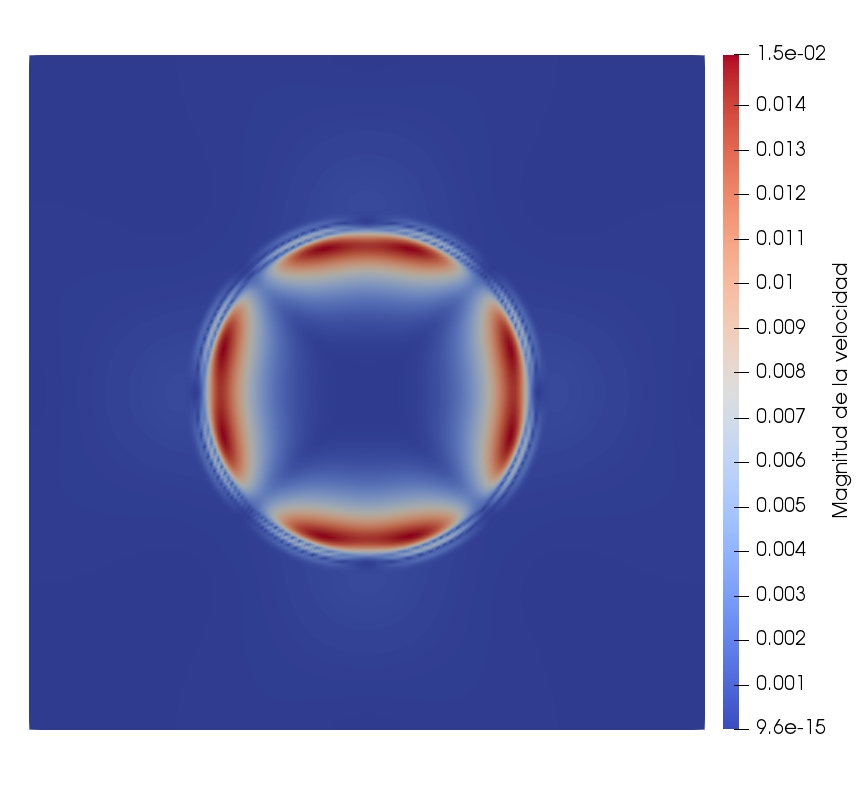
\includegraphics[width=0.95\textwidth]{FC72/Fint/Velocidad_PlanoZ_beta}
        \caption{\eq{eq:f_int_chen} con $\beta=1.25$}
    \end{subfigure}    
    \caption{Corrientes esp\'ureas en una burbuja estacionaria, obtenidas con diferentes representaciones de la fuerza de interacci\'on.}
    \label{fig:fuerza_int}
\end{figure}

El uso de una diferente aproximaci\'on para la fuerza de interacci\'on junto con el modelo MRT de Xu implica que es necesario ajustar, de manera simult\'anea, a los par\'ametros $\sigma$ y $\beta$. De esta manera, es posible lograr una disminuci\'on de las corrientes esp\'ureas mientras que se logra una buena reproducci\'on de la curva de coexistencia. En este caso, se observ\'o que la reducci\'on de las velocidades par\'asitas sobre la interfase es m\'axima para $\beta=1.25$, pero esto implica utilizar $\sigma=0.09$ para evitar inconsistencia termodin\'amica, tal como se observa en la \fig{fig:pr_sigma_beta}

\begin{figure}[ht]
	\centering
	
\includegraphics[width=0.75\textwidth]{dummy}
	\caption{Construcci\'on de Maxwell obtenida con la fuerza de interacci\'on de la \eq{eq:f_int_chen} y $\beta=1.25$}.
	\label{fig:pr_sigma_beta}
\end{figure}



\subsection{\'Angulo de contacto}

Hasta este punto, las simulaciones mostradas no incluyeron ning\'un an\'alisis exhaustivo acerca de la interacci\'on entre el fluido y las fronteras s\'olidas, ya que esta evaluaci\'on estuvo limitada a la aplicaci\'on de condiciones de contorno para la velocidad y temperaturas macrosc\'opica. Sin embargo, la descripci\'on microsc\'opica de ebullici\'on heterog\'enea requiere, adem\'as, de una representaci\'on adecuada de la interacci\'on entre las interfases y las fronteras del dominio. Esta interacci\'on puede cuantificarse a trav\'es del \'angulo de contacto, que corresponde al \'angulo en el cual la interfase fluido-fluido encuentra una fase s\'olida, y constituye una medida de la \red{mojabilidad} de la superficie. De esta forma, se considera que un fluido es \red{wetting} si el \'angulo de contacto $\theta_c < 90 \textordmasculine$, y el mismo tiende a distribuirse como una l\'amina sobre la superficie s\'olida. Por otro lado, el fluido es \red{non-wetting} si $\theta_c > 90 \textordmasculine$, de modo que tiende a formar una gota sobre la superficie.

Esta interacci\'on fluido-s\'olido y las consecuentes condiciones de mojabilidad pueden incorporarse de manera sencilla dentro de un modelo \pp{}. Tradicionalmente, suele incorporarse una fuerza de adhesi\'on entre el fluido y el s\'olido, que puede describirse mediante una forma general, similar a la de la fuerza de interacci\'on \cite{chen_critical_2014}:
\begin{equation}
	\bm{F}_{ads}= -G_w \psi(\bm{x}) \sum_{\alpha=1}^{N} w(|\bm{e}_{\alpha}|^2)\psi(\rho_w) s_i(\bm{x}+\bm{e}_{\alpha}\delta_t)\bm{e}_{\alpha},
\end{equation}
donde $s_i$ es un indicador que vale 1 para los nodos s\'olidos y 0 para los de fluido. $G_w$ y $\rho_w$ pueden ajustarse de forma conjunta o independiente para alcanzar el \'angulo de contacto deseado. Las numerosas variantes de esta t\'ecnica han sido aplicadas en la simulaci\'on de diversos problemas con interacci\'on de gotas sobre superficies (ver por ejemplo \cite{li_contact_2014, xu_three-dimensional_2015, sbragaglia_surface_2006}), o incluso en la evaluaci\'on de los efectos de mojabilidad en problemas simplificados de ebullici\'on usando esquemas de lattice Boltzmann h\'ibridos o con otros modelos de energ\'ia \cite{li_lattice_2016, ma_numerical_2019, guo_3d_2019}. Sin embargo, como se destaca en el trabajo de Hu \cite{hu_contact_2016}, este m\'etodo de fuerza de adhesi\'on sufre severas limitaciones relacionadas con la prescripci\'on del \'angulo de contacto y su influencia en la estabilidad global del modelo, lo que se refleja en la pr\'actica en acotadas condiciones de aplicabilidad. Por un lado, la conocida dificultad de cuantificar \emph{a priori} la tensi\'on superficial entre el fluido y la pared restringe la obtenci\'on de una expresi\'on clara para describir el \'angulo de contacto recuperado. Por otro lado, se pudo comprobar en las simulaciones de gotas est\'aticas sobre superficies planas que el incremento de la relaci\'on de densidades y el uso de bajas viscosidades (factores de relajaci\'on cercanos al l\'imite de estabilidad) conducen a densidades recuperadas sobre la pared con valores diferentes a las de coexistencia, mientras que se producen deformaciones no deseadas en la forma de la gota sobre la regi\'on de contacto.

Las limitaciones inherentes a los modelos de fuerza de adhesi\'on motivaron la incorporaci\'on de una representaci\'on geom\'etrica del \'angulo de contacto, similar a la utilizada por Wang \cite{wang_scheme_2013} y Hu \cite{hu_contact_2016}. Esta descripci\'on est\'a basada en la formulaci\'on presentada por Ding y Spelt \cite{ding_wetting_2007}, desarrollada para investigar las condiciones de mojabilidad en modelos multif\'asicos de interfase difusa con l\'ineas de contacto m\'oviles, resueltos con t\'ecnicas de discretizaci\'on tradicionales. En estos casos, la presencia de diferentes fases se describe a trav\'es de un par\'ametro de orden $C$, como la fracci\'on de volumen de una de las fases. Como se ejemplifica en la \fig{fig:ding_contacto}, si los contornos del par\'ametro de orden son paralelos en la interfase, el vector normal a la misma ($\bm{n_s}$) puede escribirse en t\'erminos del gradiente de $C$ como
\begin{equation}
	\bm{n_s} = \dfrac{\nabla C}{|\nabla C|}.
\end{equation}

En la l\'inea de contacto, $\bm{n_s}$ intersecta la frontera a un \'angulo de $\pi/2 - \theta_c$, donde $\theta_c$ es el \'angulo de contacto. Por lo tanto, este \'angulo puede determinarse geom\'etricamente como 
\begin{equation}
	\tan \left( \dfrac{\pi}{2} - \theta_c \right) = \dfrac{-\bm{n} \cdot \nabla C}{|\nabla C - (\bm{n}\cdot \nabla C)\bm{n}|}
	\label{eq:ding_angulo}
\end{equation}

La \eq{eq:ding_angulo} puede incorporarse a un modelo \pp{} a trav\'es del c\'alculo de densidad sobre las paredes. En particular, la fuerza de interacci\'on (Ecs. (\ref{eq:f_int_chen_0}) o (\ref{eq:f_int_chen})) sobre los nodos de la frontera puede obtenerse considerando la presencia de nodos fantasma, es decir, nodos que se encuentran dentro de la regi\'on s\'olida. En estos puntos, donde no est\'a definida la funci\'on de distribuci\'on correspondiente, la densidad necesaria para el potencial de interacci\'on puede estimarse mediante la \eq{ding_contacto}, utilizando a la densidad del fluido como par\'ametro de orden y discretizando los gradientes mediante esquemas de diferencias finitas. 

A modo de ejemplo puede considerarse una superficie plana con normal $\bm{n} = (0,0,1)$ y nodos con \'indices $(i,j,k)$. Usando esta notaci\'on, el nodo $(i,j,1)$ se encuentra sobre la superficie y el nodo $(i,j,0)$ dentro de la regi\'on s\'olida, por debajo de $(i,j,1)$ a lo largo de la normal a la superficie. De esta manera, usando diferencias centradas de segundo orden para representar los gradientes de $\rho$, es posible reescribir la \eqref{eq:ding_angulo} para calcular expl\'icitamente la densidad en el nodo fantasma $(i,j,0)$, necesaria para obtener un \'angulo de contacto $\theta_c$:
\begin{equation}
	\rho_{i,j,0} = \rho_{i,j,2} + 2 \tan \left( \dfrac{\pi}{2} - \theta_c \right) \sqrt{\left( \dfrac{\partial \rho}{\partial x} \right)_{i,i,1}^2 + \left( \dfrac{\partial \rho}{\partial y} \right)_{i,i,1}^2}  
\end{equation}




\begin{figure}[ht]
	\centering
	
\includegraphics[width=0.75\textwidth]{dummy}
	\caption{Interpretaci\'on de \'angulo y l\'inea de contacto en una interfase difusa}.
	\label{fig:ding_contacto}
\end{figure}


\section{Resultados}